\subsection{Mastering Oscilloscope Probe Compensation!}

\begin{tcolorbox}[colback=gray!10, colframe=black, title=E4A04] How is compensation of an oscilloscope probe performed?
\begin{enumerate}[label=\Alph*.]
    \item \textbf{A} A square wave is displayed, and the probe is adjusted until the horizontal portions of the displayed wave are as nearly flat as possible
    \item B A high frequency sine wave is displayed, and the probe is adjusted for maximum amplitude
    \item C A frequency standard is displayed, and the probe is adjusted until the deflection time is accurate
    \item D A DC voltage standard is displayed, and the probe is adjusted until the displayed voltage is accurate
\end{enumerate} \end{tcolorbox}

To perform compensation on an oscilloscope probe, it is essential to understand how probes interact with the oscilloscope and the signals being measured. Oscilloscope probes are used to connect the oscilloscope to the circuit under test, thereby allowing the measurement of voltage signals. However, the properties of the probe itself can affect the accuracy of these measurements, particularly at high frequencies.

Probe compensation is used to ensure that the frequency response of the probe matches that of the oscilloscope. This is important because improper compensation can lead to inaccuracies in signal representation, particularly with fast signals. 

The correct method for compensation involves displaying a square wave signal on the oscilloscope. The square wave has distinct transitions between high and low states and is the best signal to observe how a probe affects the waveform. The goal of the adjustment is to make the horizontal portions of the displayed waveform as flat as possible, which indicates that the probe's frequency response is balanced. 

Therefore, the correct answer is:
\textbf{A}

In summary, oscilloscope probe compensation is primarily concerned with ensuring that the probe can accurately reproduce signals without distortion. The method involves adjusting the probe while observing a square wave output on the oscilloscope screen.

If calculation is required, it generally pertains to understanding the impedance and frequency response of the probe rather than explicit numerical calculations for this concept. Nonetheless, if you would like to delve into impedance calculations, they would involve complex numbers to find the overall impedance of the circuit that the probe interacts with.

Below is a simplified diagram illustrating the basic concept of probe compensation, showing the adjustment process while viewing a square wave:

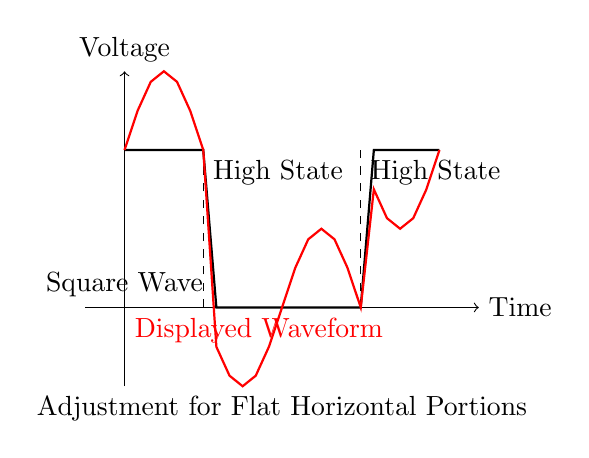
\begin{tikzpicture}
    \draw[->] (-0.5,0) -- (4.5,0) node[right] {Time};
    \draw[->] (0,-1) -- (0,3) node[above] {Voltage};
    \draw[thick] plot[domain=0:4] (\x, {ifthenelse(\x<1 || \x>3, 2, 0)}) node[midway, above] {Square Wave};
    \draw[dashed] (1,0) -- (1,2) node[below right] {High State};
    \draw[dashed] (3,0) -- (3,2) node[below right] {High State};
    \draw[thick, red] plot[domain=0:4] (\x, {ifthenelse(\x<1 || \x>3, 2, 0) + sin(180*\x)}) node[midway, below right] {Displayed Waveform};
    \node[below] at (2,-1) {Adjustment for Flat Horizontal Portions};
\end{tikzpicture}
